%
% File acl2012.tex
%
% Contact: gdzhou@suda.edu.cn
%%
%% Based on the style files for ACL2008 by Joakim Nivre and Noah Smith
%% and that of ACL2010 by Jing-Shin Chang and Philipp Koehn


\documentclass[11pt]{article}
\usepackage{acl2012}
\usepackage{times}
\usepackage{latexsym}
\usepackage{amsmath}
\usepackage{multirow}
\usepackage{url}
\usepackage{graphicx}
\DeclareMathOperator*{\argmax}{arg\,max}
\setlength\titlebox{6.5cm}    % Expanding the titlebox

\title{Multilabels for Annotation of Word Sense}

\author{First Author \\
   Affiliation / Address line 1 \\
   Affiliation / Address line 2 \\
   Affiliation / Address line 3 \\
  {\tt email@domain} \\\And
   Second Author \\
   Affiliation / Address line 1 \\
   Affiliation / Address line 2 \\
   Affiliation / Address line 3 \\
   {\tt email@domain} 
\\}

\date{}


\begin{document}
\maketitle
\begin{abstract}

\end{abstract}

\section{Introduction} % 1.0 page

Natural language data annotation typically involves drawing sharp
categorical distinctions. However, many semantic and pragmatic
dimensions of language use that are relevant or even important to
capture are either clearly not categorical, or categorization is
difficult due to a set of categories that is too numerous, too
interdependent, or too fluid.

Data annotation proceeds according to each annotator's interpretation
and application of a coding standard. The coding standard is defined
by example and by description, but may also evolve through
inter-annotator communication.

The underlying structure of language corresponding to the category
distinctions often remains to be discovered. In such cases, data
annotation is part of the larger project of linguistic research. When
a linguistic annotation can be applied consistently by different
annotators, the annotated data may be used to support the discovery
and analysis of the linguistic phenomena which correlate with the
categorizations defined by the coding standard.

We address a word sense annotation procedure in which the sense labels
are relatively numerous and potentially interdependent, and where we
% INTERDEPENDENT?
assume that in some cases an instance of a word in context can evoke a
novel sense reading (fluid senses).

In addition, data annotation is often limited by the cost of training
annotators and employing them to annotate data. More efficient means
of using annotation data thus leads to a cost savings per annotation
and thus a wider range of data that may be annotated.

Much NLP annotation involves categorical distinctions of phenomena
that can be defined by extension (examples) or intension
(description), yet where the linguistic facts that correlate with the
category distinctions remain to be discovered. Annotation guidelines
are constructed in order to train annotators in the the annotation
category definitions and examples. The annotators’ role is to annotate
language data in order to make the categorical distinctions
explicit. When the annotation is performed reliability by different
annotators, the annotated data supports the research needed for
discovery and analysis of the linguistic correlates of a phenomenon
of interest. However, many semantic and pragmatic dimensions of
language use that are relevant or even important to capture are either
clearly not categorical, or categorization is difficult due to a set
of categories that is too numerous, too interdependent, or too
fluid. In addition, it is costly to train annotators, and the use the
trained annotators for to label data. We address a word sense
annotation procedure in which the sense labels are relatively numerous
and potentially interdependent, and where we assume that in some cases
an instance of a word in context can evoke a novel sense reading
(fluid senses).

Our data consists of multilabels for each word sense instance, where
the multilabel for each instance consists of a set of labels, each
provided by a different annotator. Collecting multilabels for each
instance provides much greater dimensionality to the agreement or
disagreement among annotators on a given instance, thus highlighting
that disagreement has many gradations. In previous work, we have
argued that interannotator agreement data on many words drawing from
the same annotators indicates that the trained annotators can perform
the general procedure reliably, but that reliability can still be low,
depending on the word. In our previous work, we compared performance
of an unsupervised learning method to learn an unknown (hidden) {\it
true} label from multilabels of different sizes, and where the
labelers were trained or not. In separate work on multilabel
annotation with multiple labelers, we showed the use of a hierarchical
Bayesian model of annotation to estimate annotator quality and item
difficulty from the observed sets of multilabels. Here we will build
on both lines of investigation to compare different estimates of
annotator accuracy. We also examine other sources of uncertainty
regarding word sense multilabels, such as item difficulty.

\section{Related Work} % 0.25 page

Multilabels have been used in machine learning for the problem of
reducing the cost of label acquisition, or improving label accuracy of
manual labels, or both~\cite{snowEtAl08,shengEtAl_2008}. For this type
of multilabel, it is assumed that there is a true label and that each
annotator who contributes to a multilabel for each instance has an
unknown probability of being correct that is (sometimes much) less
than 100\%.

Multilabels have also been used in machine learning approaches to
address the problem of how to assign instances to multiple
classes~\cite{tsoumakas&katakis_2007,boutellEtAl_2004,mccallum_1999}.
The assumption behind these approaches is that there are instances
that cannot be assigned a single label because they belong partly to
one class and partly to another. For a multilabel to represent
simultaneous membership of an instance in multiple classes, each class
represented in the multilabel should be a {\it true} class. {for
example?} For instances where a given word seems to have properties of
more than one sense in a given sense inventory, a multilabel can
represent all the senses the word exhibits. {give examples from LRE
paper for 'fair' and 'quiet'} An issue that arises with this sort of
multilabel is how to arrive at the {\it true} multilabel for unlabeled
data.

Word meaning has been variously represented in lexicography,
linguistics and computational linguistics. Approaches include: a
hierarchy of sense definitions (as in conventional dictionaries),
WordNet's ordered inventory of sets of synonyms plus sense
definitions~\cite{millerEtAl93}, one or more components of a
conceptual frame as in FrameNet~\cite{fillmoreEtAl03}, a decomposition
into logical predicates and operators~\cite{dowty79}, a cluster of
sentences where a word form in all of them has the same meaning (as
argued for in~\cite{kilgarriff97}), or some combination of the above.
Recent work by Erk and colleagues builds on the view that a sense can
be defined as the contexts it occurs in~\cite{kilgarriff97}, or more
specifically as regions in a vector space model~\cite{erk09}. We rely
on WordNet senses for our annotation tasks. Since all sentences for a
given lemma are annotated at the same time, and the WordNet senses
include glosses along with definitions, our annotation task is similar
to clustering instances by their similarity to the glosses.

\section{Word Sense and Multilabels} % 0.5 page

WordNet is a large lexical resource that has been used for a
large-scale word sense annotation project as part of a project to
create a Manually Annotated SubCorpus (MASC) of the Open American
National Corpus (OANC)~\cite{ideEtAl10}. The word sense corpus,
described more fully in ~\cite{passonneauEtAl12}, consists of a
sentence corpus from MASC (and supplemented where needed from the OANC
for more lower frequency words) with approximately 1,000 sentences
each for 100 words representing nouns, verbs and adjectives. All
instances of the 100 words have been annotated with WordNet senses.
The average number of WordNet senses is about 8 per word. For each
word, about 900 instances were annotated by a single annotator from a
pool of 10 trained annotators, and the remaining 100 by four
annotators. We have 10 words that were annotated by six trained
annotators, and also by 14 mechanical turkers for 3 of the words. We
use this sample of 1000 instances to illustrate the Bayesian model for
estimating annotator quality.

\section{Annotator Quality and Multilabels} % 1 page

Much work on annotation measures reliability of annotators, meaning
their consistency on the annotation task, using pairwise agreement or
an agreement coefficient such as $\kappa$~\cite{cohen60} or
$\alpha$~\cite{krippendorff80}. These metrics cannot rank annotators
by their quality, they can only be used to rank annotators by their
level of agreement with other annotators. Annotator quality as
estimaged by graphical models such as GLAD~\cite{whitehillEtAl-2009}
differs from measures of interannotator agreement in that it is a
score assigned to an individual annotator, but we do find a strong
correlation of average interannotator agreement and GLAD annotator
quality scores on some senses.

Five trained annotators who annotasted 99 instances of the adjective
{\it fair} in column 1. {\it Fair} has 10 WordNet senses, 6 of which
were used in this dataset. Because GLAD learns binary classifiers, we
converted the $k=6$ labels used by annotators to $k=2$, to investigate
each WordNet sense. Sense 1 occurs by at least one annotator on 52 of
the 99 instances. Table~\ref{tab:fair-101-glad-kripp} shows the five
annotators, and two scores that give the same rank to the annotators.
The first is $\alpha$~\cite{krippendorff80}, computed for each
annotator with each other annotator, then averaged over all the pairs
for that annotator to get. The second is the GLAD annotator accuracy
score. The full paper will discuss the correlations among different
annotator scores within words and across words.

%% fair 101 MASC
%% ann    Glad alpha    avg Kripp Alpha
%% 101    0.8135 4       0.6055 4
%% 102    0.6825 5       0.5573 5
%% 105    1.2465 3       0.6770 3
%% 107    1.3237 2       0.6815 2
%% 108    1.3669 1       0.7028 1

\begin{figure}
\begin{center}
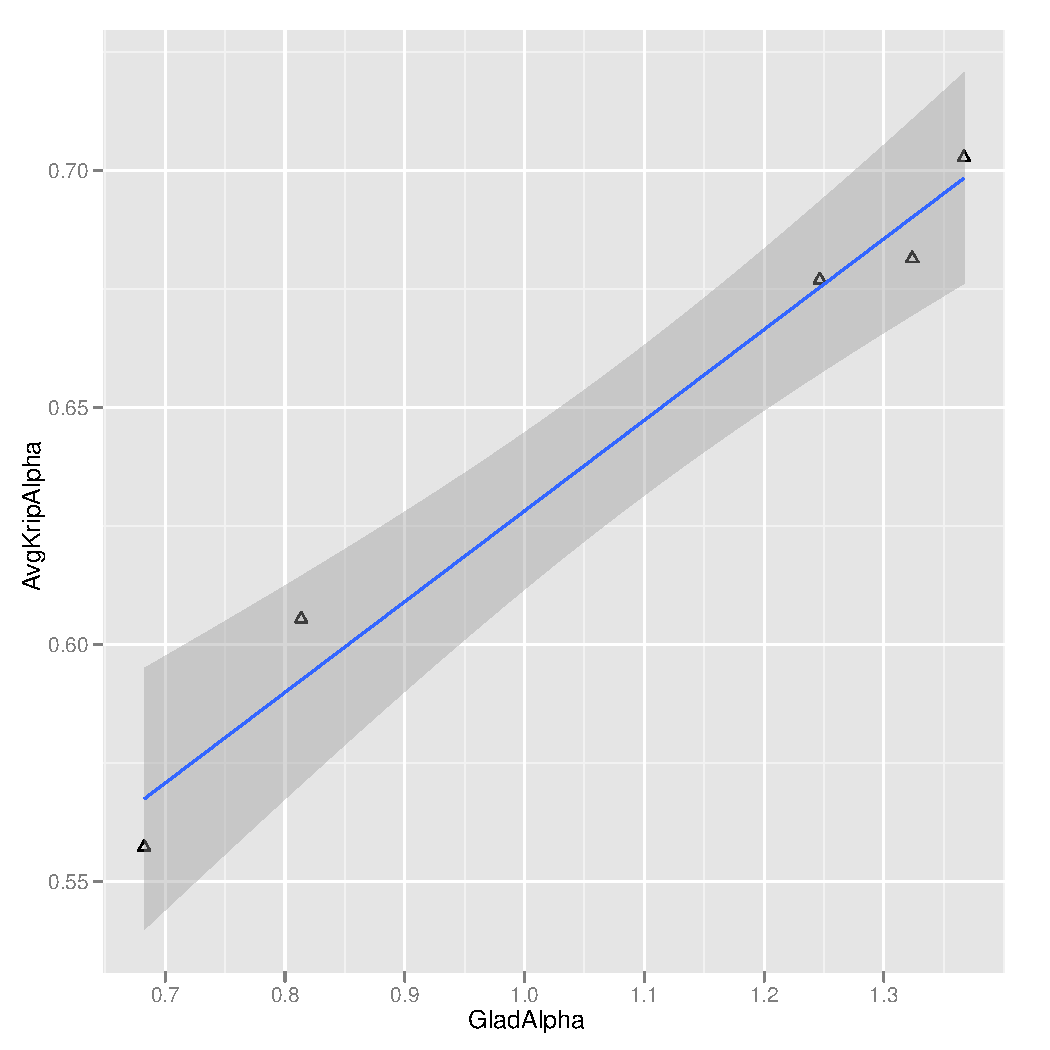
\includegraphics[width=0.5\textwidth]{img/GladVsKripp.pdf}
\end{center}
\caption{Average Krippendorf $\alpha$ versus Glad $\alpha$ for five
annotators for the word {\it fair}.  The line is the linear regression
fit.}
\end{figure}

\begin{figure*}
\includegraphics[width=\textwidth]{img/fair-response.pdf}
\caption{Estimated annotator response to given categorical
inputs.}
\end{figure*}

\section{Item Difficulty and Multilabels}


\section{Conclusion} % 0.25 page

\section*{Acknowledgments}
\bibliographystyle{acl2012}
\bibliography{wordsense-multilabels}
\end{document}
